\documentclass{article}

\usepackage{tikz} 
\usetikzlibrary{automata, positioning, arrows} 

\usepackage{amsthm}
\usepackage{amsfonts}
\usepackage{amsmath}
\usepackage{amssymb}
\usepackage{fullpage}
\usepackage{color}
\usepackage{parskip}
\usepackage{hyperref}

  \hypersetup{
    colorlinks = true,
    urlcolor = blue,       % color of external links using \href
    linkcolor= blue,       % color of internal links 
    citecolor= blue,       % color of links to bibliography
    filecolor= blue,        % color of file links
    }
    
\usepackage{listings}

\definecolor{dkgreen}{rgb}{0,0.6,0}
\definecolor{gray}{rgb}{0.5,0.5,0.5}
\definecolor{mauve}{rgb}{0.58,0,0.82}

\lstset{frame=tb,
  language=haskell,
  aboveskip=3mm,
  belowskip=3mm,
  showstringspaces=false,
  columns=flexible,
  basicstyle={\small\ttfamily},
  numbers=none,
  numberstyle=\tiny\color{gray},
  keywordstyle=\color{blue},
  commentstyle=\color{dkgreen},
  stringstyle=\color{mauve},
  breaklines=true,
  breakatwhitespace=true,
  tabsize=3
}

\newtheoremstyle{theorem}
  {\topsep}   % ABOVESPACE
  {\topsep}   % BELOWSPACE
  {\itshape\/}  % BODYFONT
  {0pt}       % INDENT (empty value is the same as 0pt)
  {\bfseries} % HEADFONT
  {.}         % HEADPUNCT
  {5pt plus 1pt minus 1pt} % HEADSPACE
  {}          % CUSTOM-HEAD-SPEC
\theoremstyle{theorem} 
   \newtheorem{theorem}{Theorem}[section]
   \newtheorem{corollary}[theorem]{Corollary}
   \newtheorem{lemma}[theorem]{Lemma}
   \newtheorem{proposition}[theorem]{Proposition}
\theoremstyle{definition}
   \newtheorem{definition}[theorem]{Definition}
   \newtheorem{example}[theorem]{Example}
\theoremstyle{remark}    
  \newtheorem{remark}[theorem]{Remark}

\title{CPSC-354 Report}
\author{Sarah Yoon  \\ Chapman University}

\date{\today} 

\begin{document}

\maketitle

\begin{abstract}
This report describes the concepts and techniques learned throughout the course, specifically Lean, proofs, and lambda calculus. 
Each week goes through a specific topic within the general concepts. The purpose of exploring all these topics is to get familiar 
with the core principles of programming languages. 

\end{abstract}

\setcounter{tocdepth}{3}
\tableofcontents

\section{Introduction}\label{intro}
The very fundementals of programming languages (syntax, interpretation, etc) are based on math and logic. The report goes over 
what was learned each week. The goal of exploring each topic is to understand what is takes to construct a programming language (e.g. recursion, AST).
The report goes in order of what was learned first to the most recent. It first delves into mathmatical proofs/Lean and then slowly starts connecting 
to the concepts of programming languages. 
\section{Week by Week}\label{homework}

\subsection{Week 1}

\subsubsection*{Notes}
Learned about some tactics and theorems

rfl: a tactic that proves theorems that take the form of X = X \\
rw: a tactic that rewrites a proof\\
one\_eq\_succ\_zero: a theorem that proves 1 = succ 0 (there are also other similar existing theorems like two\_eq\_succ\_one and so on)\\
add\_zero: a theorem that proves a + 0 = a.\\
add\_succ: a theorem that proves a + succ b = succ(a + b)\\
succ\_eq\_add\_one: a theorem that proves succ a = a + 1\\

\subsubsection*{Homework}
Problem 5: \\
a b c are in the set of natural numbers. \\
Prove that both sides are equal to each other. \\
a + (b + 0) + (c + 0) = a + b + c \\
rw [add\_zero] - uses the add\_zero theorem to prove that b + 0 = b \\
This is rewritten to: \\
a + b + (c + 0) = a + b + c \\
rw [add\_zero] - this is done again to prove that c + 0 = c \\ 
This is rewritten to: \\
a + b + c = a + b + c \\
rfl - this proves that both sides that look the same are equal to each other \\

Problem 6: \\
This is the same problem as 5 but will be approached in a different manner. \\
a + (b + 0) + (c + 0) = a + b + c \\
rw [add\_zero c] - specifically applies the add\_zero theorem to c, making c + 0 into c \\
This is rewritten to: \\ 
a + (b + 0) + c = a + b + c \\
rw [add\_zero b] - specifically applies the add\_zero theorem to b, making b + 0 into b \\
This is rewritten to: \\ 
a + b + c = a + b + c \\
rfl - this proves that both sides that look the same are equal to each other \\

Problem 7: \\
n is in the set of natural numbers. \\
Prove that both sides are equal to each other. \\
succ n = n + 1
rw[one\_eq\_succ\_zero] - rewrite 1 into successor 0
This is rewritten to: \\ 
succ n = n + succ 0 \\
rw[add\_succ] - uses the add\_succ theorem to change n + succ 0 into succ(n + 0) \\
This is rewritten to: \\ 
succ n = succ (n + 0) \\
rw[add\_zero] - uses the add\_zero theorem to prove that n + 0 = n \\
This is rewritten to: \\ 
succ n = succ n \\
rfl - this proves that both sides that look the same are equal to each other \\

Problem 8: \\
Prove that both sides are equal to each other. \\
2 + 2 = 4 \\
rw[two\_eq\_succ\_one] - rewrites 2 into succ 1 \\
This is rewritten to: \\ 
succ 1 + succ 1 = 4 \\
rw[one\_eq\_succ\_zero] - rewrites 1 into succ 0 \\
This is rewritten to: \\ 
succ (succ 0) + succ (succ 0) = 4 \\
rw[four\_eq\_succ\_three] - rewrites 4 into succ 3 \\
This is rewritten to: \\ 
succ (succ 0) + succ (succ 0) = succ 3 \\
rw[three\_eq\_succ\_two] - rewrites 3 into succ 2 \\
This is rewritten to: \\ 
succ (succ 0) + succ (succ 0) = succ (succ 2) \\
rw[two\_eq\_succ\_one] - rewrites 2 into succ 1 \\
This is rewritten to: \\ 
succ (succ 0) + succ (succ 0) = succ (succ (succ 1)) \\
rw[one\_eq\_succ\_zero] - rewrites 1 into succ 0 \\
This is rewritten to: \\ 
succ (succ 0) + succ (succ 0) = succ (succ (succ (succ 0))) \\
rw[add\_succ] - changes succ (succ 0) + succ (succ 0) into succ (succ (succ 0) + succ 0) \\
This is rewritten to: \\ 
succ (succ (succ 0) + succ 0) = succ (succ (succ (succ 0))) \\
rw[add\_succ] - changes succ (succ (succ 0) + succ 0) into succ (succ (succ (succ 0) + 0)) \\
This is rewritten to: \\ 
succ (succ (succ (succ 0) + 0)) = succ (succ (succ (succ 0))) \\
rw[add\_zero] - changes succ (succ 0) + 0 into \\
This is rewritten to: \\ 
succ (succ (succ (succ 0))) = succ (succ (succ (succ 0))) \\ 
rfl - this proves that both sides that look the same are equal to each other \\

For level 5: 
add\_zero is a Lean proof that a + 0 = a (a representing any number). In mathematics, there are laws for arithemic. One of them 
is called the identity which applies to addition and multiplication. For addition, it states that m + 0 = m = 0 + m. This is the
exact same as the Lean proof, a + 0 = a, which can also be written as a = 0 + a.

%In case you want to draw automata in Latex, you can use the tikz %package. Here is an example of a simple automaton:
%
%\begin{tikzpicture}[shorten >=1pt,node distance=2cm,on grid,auto] 
%  \node[state] (q_1)   {$q_1$}; 
%  \node[state] (q_2) [above right=of q_1] {$q_2$}; 
%  \node[state] (q_3) [below right=of q_2] {$q_3$}; 
%   \path[->] 
%   (q_1) edge  node {0} (q_2)
%         edge  node [swap] {1} (q_3)
%   (q_2) edge  node  {1} (q_3)
%         edge [loop above] node {0} ()
%   (q_3) edge [loop below] node {0,1} ();
%\end{tikzpicture}
%
%By the way, GPT-4 is quite good at outputting tikz code.

\subsubsection*{Comments and Questions}
Learning the root of mathematics is very eye-opening, and I am confident it will be the same for programming languages. 
It provides another perspective for elementary functions like 2 + 2 equals 4, which is different from just knowing it through memorization. 
I feel as though this is why people have been able to expand mathematically. This makes me wonder: how can looking through the core of 
programming help us better current languages (e.g. python, rust)?
%I expect you to read the lecture notes. 

\subsection{Week 2}

\subsubsection*{Notes}
Recursion as a concept using the Towers of Hanoi:
It is broken down into:
 moving a tower of n disks from x to y
 moving a tower of n+1 disks when it is already known how to move a tower of n disks
The algorithm is made up of a bunch of "pushs" and "pops"
The logic overall is a bunch of back and forth movement of the disks 

Lean:
induction proof with: induction n with d hd
succ\_add: proves that succ a + b = succ (a + b)
add\_comm x y: proves that x + y = y + x
add\_assoc: proves that a + b + c = a + (b + c)
add\_right\_comm a b c: proves that a + b + c = a + c + b 

\subsubsection*{Homework}
Problem 1:\\
n is in the natural number set\\
Prove 0 + n = n.\\
induction n with d hd - starting a proof by induction\\
Now our first goal is:\\
0 + 0 = 0\\
rw[add\_zero] - proves that 0 + 0 = 0\\
This is rewritten to:\\
0 = 0\\
rfl - this proves that both sides that look the same are equal to each other \\
Now, we prove our second goal\\
hd: 0 + d = d\\
0 + succ d = succ d \\
rw[add\_succ] - proves that 0 + succ d = succ (0 + d)\\
This is rewritten to:\\
succ (0 + d) = succ d\\
rw[hd] - this replaces 0 + d with d\\
This is rewritten to:\\
succ d = succ d\\
rfl - this proves that both sides that look the same are equal to each other \\

Problem 2:\\
a b is in the set of natural numbers\\
Prove succ a + b = succ (a + b)\\
inductin b with d hd - starting a proof by induction\\
Now our first goal is:\\
succ a + 0 = succ (a + 0)\\
rw[add\_zero] - proves that succ a + 0 = succ a\\
This is rewritten to:\\
succ a = succ(a + 0)\\
rw[add\_zero] - proves that succ (a + 0) = succ a\\
This is rewritten to:\\
succ a = succ a\\
rfl - this proves that both sides that look the same are equal to each other \\
Now, we prove our second goal\\
hd: succ a + d = succ (a + d)\\
succ a + succ d = succ (a + succ d)\\
rw[add\_succ] - proves that succ a + succ d = succ (succ a + d)\\
This is rewritten to:\\
succ (succ a + d) = succ (a + succ d)\\
rw[hd] - this replaces succ a + d with succ (a + d)\\
This is rewritten to:\\
succ (succ (a + d)) = succ (a + succ d)\\
rw[add\_succ] - proves that succ (a + succ d) = succ (succ (a + d))\\
This is rewritten to:\\
succ (succ (a + d)) = succ (succ (a + d))\\
rfl - this proves that both sides that look the same are equal to each other \\

Problem 3:\\
a b is in the set of natural numbers\\
Prove a + b = b + a\\
induction b with hd - starting a proof by induction\\
Now our first goal is:\\
a + 0 = 0 + a\\
rw[zero\_add] - proves that 0 + a = a\\
This is rewritten to:\\
a + 0 = a\\
rw[add\_zero] - proves that a + 0 = a\\
This is rewritten to:\\
a = a\\
rfl - this proves that both sides that look the same are equal to each other \\
Now, we prove our second goal\\
n\_ih: a + hd = hd + a\\
a + succ hd = succ hd + a\\
rw[add\_succ] - proves that a + succ hd = succ (a + hd)\\
This is rewritten to:\\
succ (a + hd) = succ hd + a\\
rw[succ\_add] - proves that succ hd + a = succ (hd + a)\\
This is rewritten to:\\
succ (a + hd) = succ (hd + a)\\
rw[n\_ih] - replaces succ (a + hd) with succ (hd + a)\\
This is rewritten to:\\
succ (hd + a) = succ (hd + a)\\
rfl - this proves that both sides that look the same are equal to each other \\

Problem 4:\\
a b c is in the set of natural numbers\\
Prove a + b + c = a + (b + c)\\
induction a with hd - starting a proof by induction\\
Now our first goal is:\\
0 + b + c = 0 + (b + c)\\
rw[zero\_add] - proves that 0 + b = b\\
This is rewritten to:\\
b + c = 0 + (b + c)\\
rw[zero\_add] - proves that 0 + (b + c) = b + c\\
This is rewritten to:\\
b + c = b + c\\
rfl - this proves that both sides that look the same are equal to each other \\
Now, we prove our second goal\\
n\_ih: hd + b + c = hd + (b + c)\\
succ hd + b + c = succ hd + (b + c)\\
rw[succ\_add] - proves that succ hd + b + c = succ (hd + b) + c\\
This is rewritten to:\\
succ (hd + b) + c = succ hd + (b + c)\\
rw[succ\_add] - proves that succ (hd + b) + c = succ (hd + b + c)\\
This is rewritten to:\\
succ (hd + b + c) = succ hd + (b + c)\\
rw[n\_ih] - replaces succ (hd + b + c) with succ (hd + (b + c))\\
This is rewritten to:\\
succ (hd + (b + c)) = succ hd + (b + c)\\
rw[succ\_add] - proves succ hd + (b + c) = succ (hd + (b + c))\\
This is rewritten to:\\
succ (hd + (b + c)) = succ (hd + (b + c))\\
rfl - this proves that both sides that look the same are equal to each other \\

Problem 5:\\
a b c is in the set of natural numbers\\
Prove a + b + c = a + c + b\\
induction c with hd - starting a proof by induction\\
Now our first goal is:\\
a + b + 0 = a + 0 + b\\
rw[add\_zero] - proves that b + 0 = b\\
This is rewritten to:\\
a + b = a + 0 + b\\
rw[add\_zero] 0 proves that a + 0 = a\\
This is rewritten to:\\
a + b = a + b\\
rfl - this proves that both sides that look the same are equal to each other \\
Now, we prove our second goal\\
n\_ih: a + b + hd = a + hd + b\\
a + b + succ hd = a + succ hd + b\\
rw[add\_succ] - proves that a + b + succ hd = succ (a + b + hd)\\
This is rewritten to:\\
succ (a + b + hd) = a + succ hd + b\\
rw[add\_succ] - proves that a + succ hd + b = succ (a + hd) + b\\
This is rewritten to:\\
succ (a + b + hd) = succ (a + hd) + b\\
rw[succ\_add] - proves that succ (a + hd) + b = succ (a + hd + b)\\
This is rewritten to:\\
succ (a + b + hd) = succ (a + hd + b)\\
rw[n\_ih] - replaces a + b + hd with a + hd + b\\
This is rewritten to\\
succ (a + hd + b) = succ (a + hd + b)\\
rfl - this proves that both sides that look the same are equal to each other \\

Problem 5 Proof in Mathematics:\\
a + b + c =  a + (b + c)\\
0 + b + c = 0 + (b + c) - Basis\\
b + c = 0 + (b + c) - Addition Identity\\
b + c = b + c - Addition Identity\\
Inductive Step:\\
k + b + c = k + (b + c)\\
The goal is to prove that Sk + b + c = Sk + (b + c)\\
S(k + b + c) = Sk + (b + c) - Definition of Addition\\
S(k + b + c) = S(k + (b + c)) - Definition of Addition\\
S(k + (b + c)) = S(k + (b + c)) - Inductive Hypothesis\\
Therefore, by the Axiom of induction a + b + c =  a + (b + c) for all a in the natural numbers set\\
\\
Math to Lean\\
Basis: induction a with hd\\
Addition Identity: zero\_add\\
Definition of Addition: succ\_add\\
Inductive Hypothesis: n\_ih\\

\subsubsection*{Comments and Questions}
The Towers of Hanoi reminded me of solving certain problems by simply using recursion. 
I also remember applying this method to the Fibonacci sequence. This makes me wonder 
how it transfers to math. How does recursion 
appear in mathematics or, specifically, in Lean?

\subsection{Week 3}

\subsubsection*{Homework}
\href{https://github.com/sarah-yoon/CPSC354_Week3/blob/main/README.md}{Week 3 Assignment}\\
\subsubsection*{Comments and Questions}
My literature review is about the cause for many different programming languages, the abstraction of them in the future, and what needs future ones would need to fulfill. 
I found that languages evolved depending on the different needs and users over time. For instance, Domain-specific languages were created to meet specific needs. SQL, being one of them, was created to interact with databases.
Within the topic of abstraction, PLs are bound to become higher level to not worry about lower-level implementation. Examples of the current progress towards abstraction would be AI-assisted programming and declarative programming. 
However, abstraction will not change the usage of current languages like Java, Python, and C++ in the foreseeable future. These languages have made a huge impact and it is shown through their extensive ecosystems and sheer amount of existing codebases. On the other hand, some specific areas use newer languages like Rust and Kotlin. They fulfill more modern needs like memory safety and developer productivity.
Future programming languages would need to deal with challenges like security, AI, and concurrency.

\subsection{Week 4}
\subsubsection*{Homework}
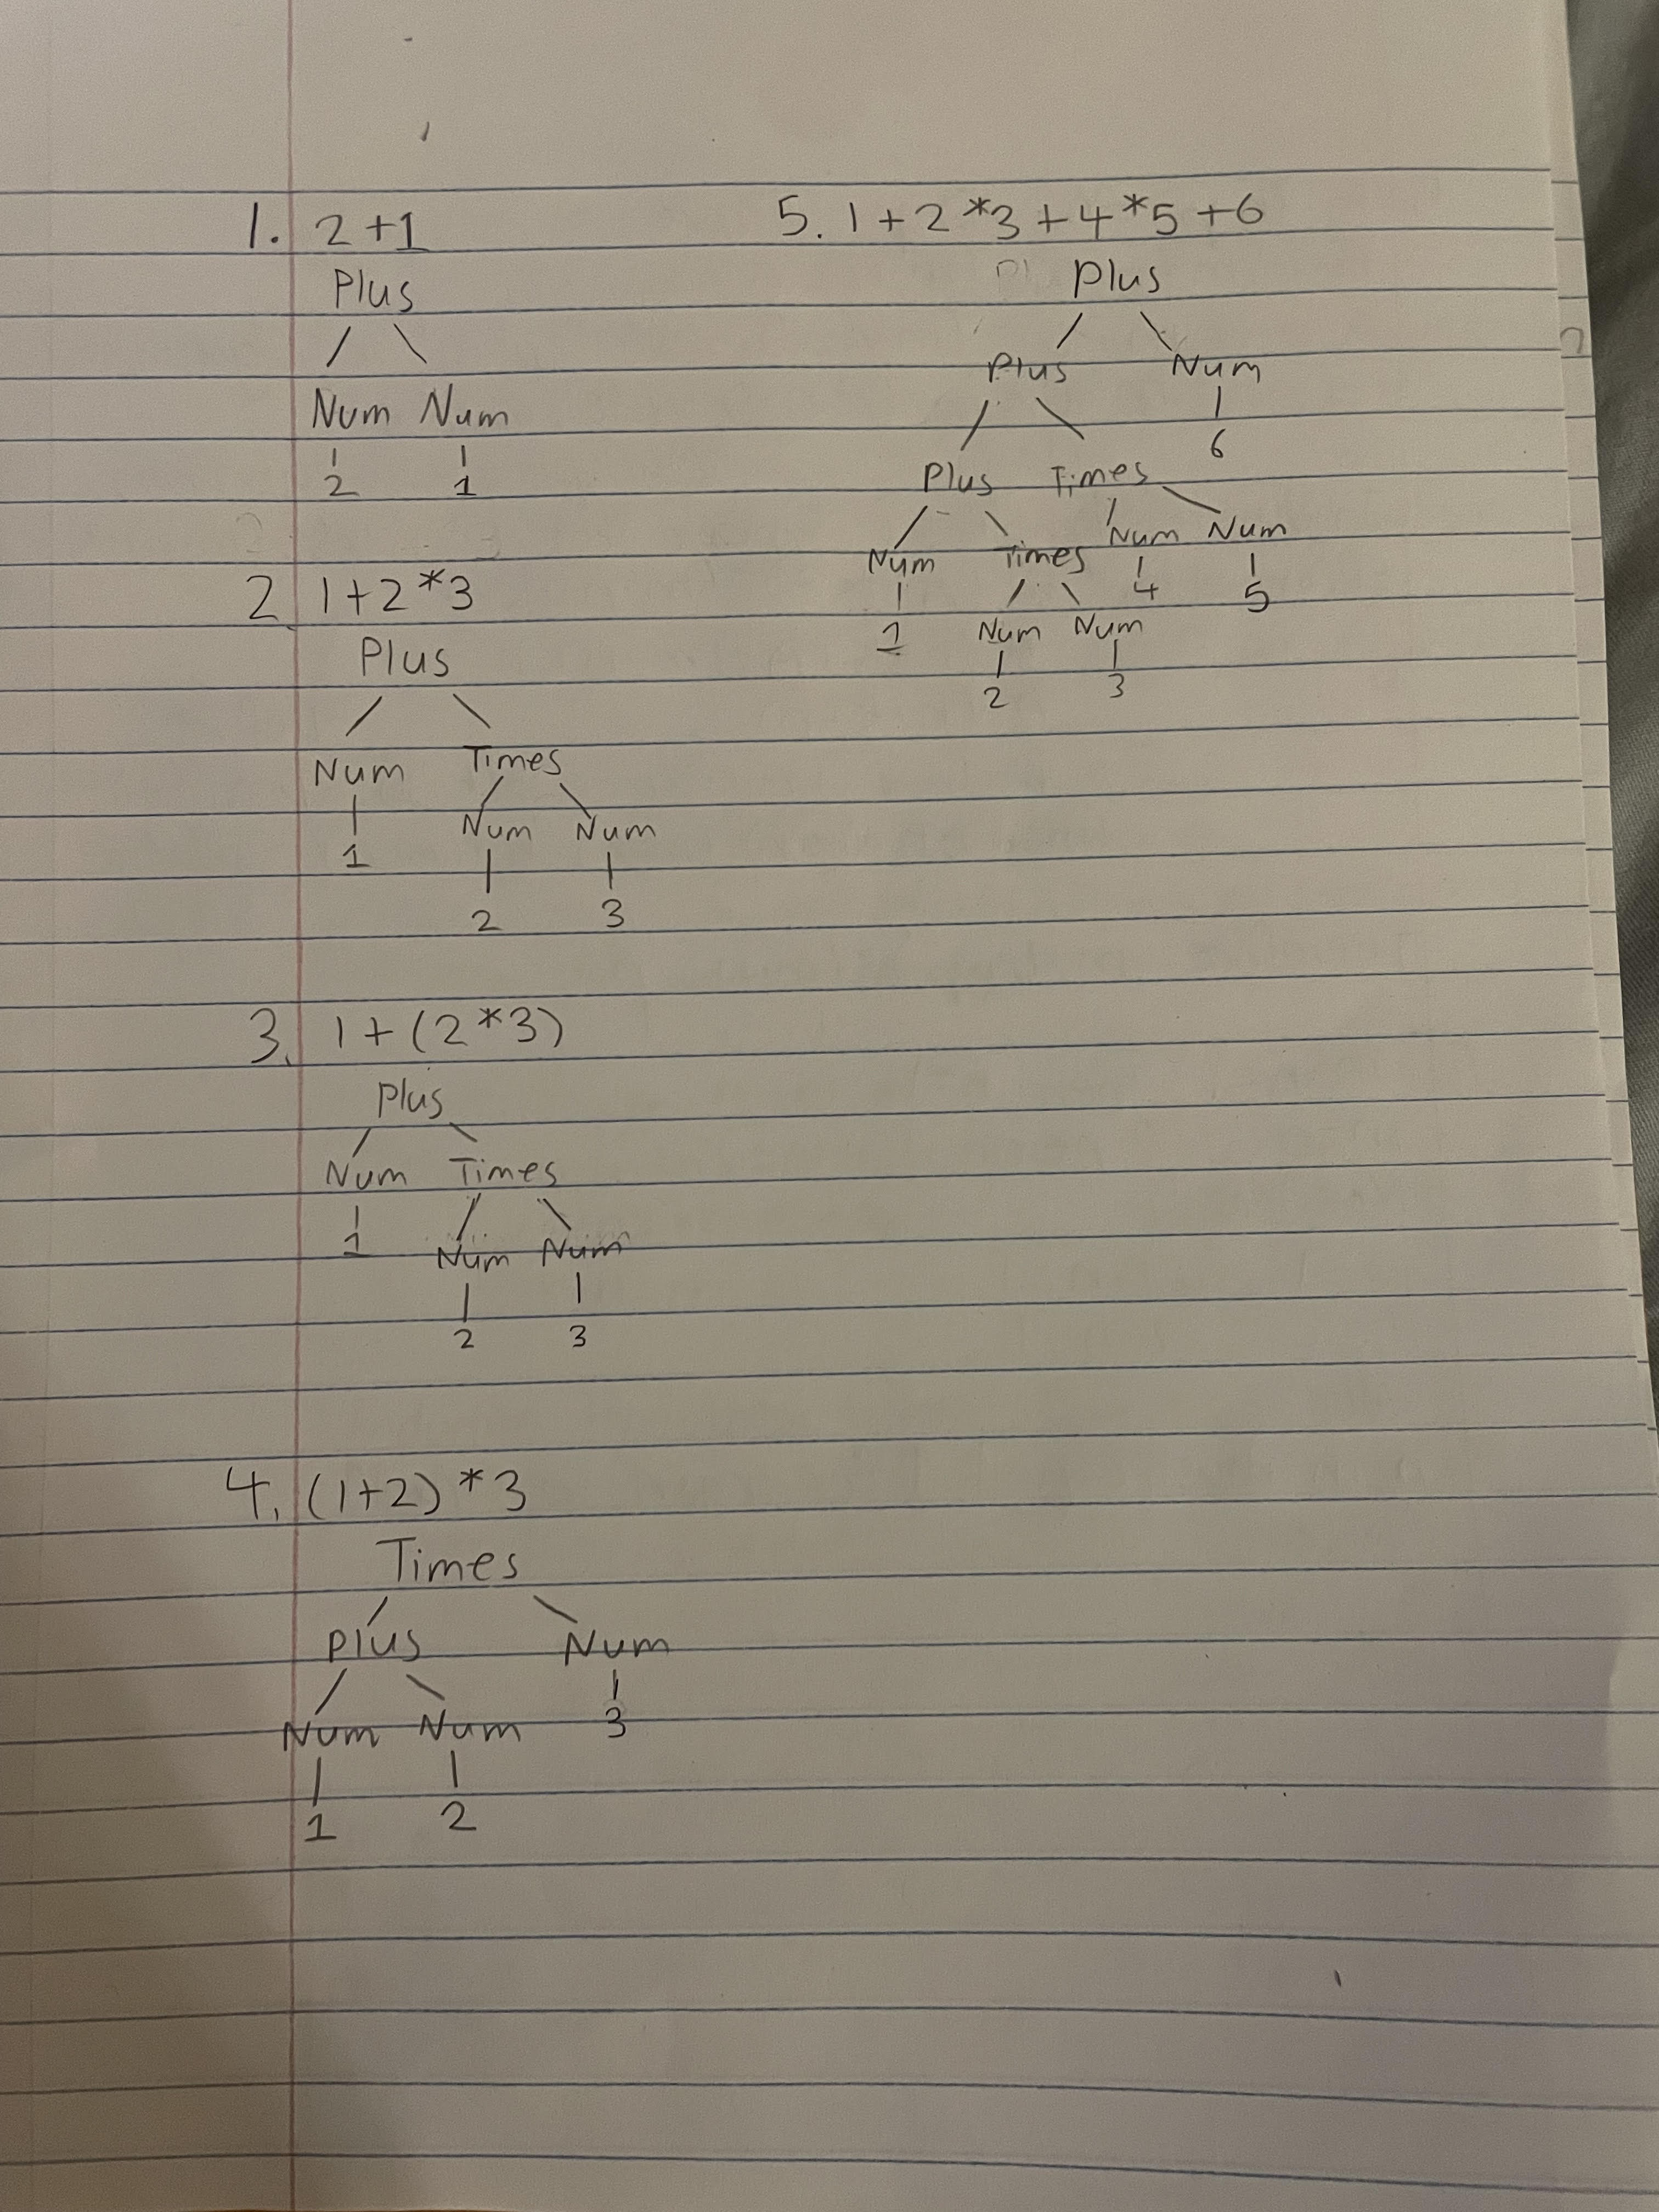
\includegraphics[scale=0.1]{parsing.jpg}
\subsubsection*{Comments and Questions}
Parsing seemed to work really great with expressions. In general, is parsing a good strategy when it comes to breaking things down?

\subsection{Week 5}
\subsubsection*{Notes}
exact -conclusion of a proof\\
Operator: $\land$ -Logical And\\
Example: $A \land B$ -A and B\\
and\_into -takes two pieces of evidence and combines it into one\\
have -adds new assumptions to the proof\\

\subsubsection*{Homework}
Problem 1:\\
exact todo\_list\\

Problem 2:\\
exact and\_intro p s \\

Problem 3:\\
exact ⟨⟨a,i⟩,⟨o,u⟩⟩\\

Problem 4:\\
have p := and\_left vmS\\
exact p\\

Problem 5:\\
have q := and\_right h\\
exact q\\

Problem 6:\\
have a := and\_left h1\\
have u := and\_right h2\\
exact ⟨a, u⟩\\

Problem 7:\\
have h1 := h.left \\
have h2 := h1.right \\
have h3 := h2.left \\
have h4 := h3.left \\
have h5 := h4.right \\
exact h5 \\

Problem 8:\\
have h1 := h.left \\
have a := h1.right\\
have h2 := h1.left\\
have p := h2.left\\
have s := h2.right\\
have h3 := h.right\\
have h4 := h3.right\\
have h5 := h4.left\\
have c := h5.left\\

In mathmatical proof:\\
If $((P \land S) \land A) \land ¬I \land (C \land ¬O) \land ¬U$ then $A \land C \land P \land S$. \\
Proof:\\
(1)\\
$((P \land S) \land A) \land ¬I \land (C \land ¬O) \land ¬U$\\
assumption\\

(2)\\
$(P \land S) \land A$\\
and\_left (1)

(3)\\
A\\
and\_right (2)\\

(4)\\
$(P \land S)$\\
and\_left (2)\\

(5)\\
P\\
and\_left (4)\\

(6)\\
S\\
and\_right (4)\\

(7)\\
$¬I \land (C \land ¬O) \land ¬U$\\
and\_right (1)\\

(8)\\
$(C \land ¬O) \land ¬U$\\
and\_right (7)\\

(9)\\
$C \land ¬O$\\
and\_left (8)\\

(10)\\
C\\
and\_left (9)\\

(11)\\
$A \land C \land P \land S$\\
and\_intro (3)(10)(5)(6)\\

\subsubsection*{Comments and Questions}
How does lean help with problem solving when it comes to programming?\\

\subsection{Week 6}
\subsubsection*{Homework}
Problem 1:\\
have b := bakery\_service p\\
exact b\\

Problem 2:\\
exact fun h : $C =>$ h\\

Problem 3:\\
exact fun $h =>$ and\_intro h.right h.left\\

Problem 4:\\
exact fun h : $C =>$ have a : A := h1 h; h2 a\\

Problem 5:\\
have q : Q := h1 p\\
have t : T := h3 q\\
exact h5 t\\
               
Problem 6:\\
exact fun c : $C =>$\\
  fun d : $D =>$\\
    have cd : $C \land D$ := ⟨c, d⟩;\\
    h cd    \\
    
Couldn't finish...

\subsubsection*{Comments and Questions}
Solving lean logic game is a simple view into proving theorems and the foundations of programming languages. When it comes to the lambda problems specifically, how do real-world challenges complicate the applications of lambda?

\subsection{Week 7}
\subsubsection*{Homework}
1.\\
\[
((\lambda m. \lambda n. m \, n) \, (\lambda f. \lambda x. f \, (f \, x))) \, (\lambda f. \lambda x. f \, (f \, (f \, x)))
\]

\[
((\lambda m. \lambda n. m \, n) \, (\lambda f. \lambda x. f \, (f \, x))) \rightarrow \lambda n. (\lambda f. \lambda x. f \, (f \, x)) \, n
\]

\[
(\lambda f. \lambda x. f \, (f \, x)) \, n \rightarrow \lambda x. n \, (n \, x)
\]

\[
(\lambda n. \lambda x. n \, (n \, x)) \, (\lambda f. \lambda x. f \, (f \, (f \, x)))
\]

\[
(\lambda n. \lambda x. n \, (n \, x)) \, (\lambda f. \lambda x. f \, (f \, (f \, x))) \rightarrow \lambda x. (\lambda f. \lambda x. f \, (f \, (f \, x))) \, ((\lambda f. \lambda x. f \, (f \, (f \, x))) \, x)
\]

\[
(\lambda f. \lambda x. f \, (f \, (f \, x))) \, x \rightarrow \lambda x. x \, (x \, (x \, x))
\]

\[
\lambda x. (\lambda f. \lambda x. f \, (f \, (f \, x))) \, (\lambda x. x \, (x \, (x \, x)))
\]

\[
(\lambda f. \lambda x. f \, (f \, (f \, x))) \, (\lambda x. x \, (x \, (x \, x))) \rightarrow \lambda x. (\lambda x. x \, (x \, (x \, x))) \, ((\lambda x. x \, (x \, (x \, x))) \, x)
\]

\[
(\lambda x. x \, (x \, (x \, x))) \, x \rightarrow x \, (x \, (x \, x))
\]

\[
\lambda x. (\lambda x. x \, (x \, (x \, x))) \, (x \, (x \, (x \, x)))
\]

\[
(\lambda x. x \, (x \, (x \, x))) \, (x \, (x \, (x \, x))) \rightarrow (x \, (x \, (x \, x))) \, ((x \, (x \, (x \, x))) \, ((x \, (x \, (x \, x))) \, (x \, (x \, (x \, x))))
\]

2.\\
The lambda term implements addition on natural numbers. It is done by combing two Church numerals. It carries out addition by counting the the total number of times the function is being applied. 
\subsubsection*{Comments and Questions}
Can church numerals be used to represent recursive functions/processes?

\subsection{Week 8}
\subsubsection*{Homework}
Answers on week 9
\subsubsection*{Comments and Questions}
When it comes to evaluation strategies in lambda calculus, what are the trade-offs? How do these strategies affect performance and accuracy in a practical implementation?

\subsection{Week 9}
\subsubsection*{Homework}
2. a is applied to b, which leads to (ab). Then, (ab) is applied to c, resulting in ((ab)c). Finally, ((ab)c) is applied to d, which leads to (((ab)c)d). (a) reduces to a it's already in its simplest form.

3.When substituting a variable, wall instances of that variable are replaced. However, if the variable being substituted for is also bound, the meaning of the expression is changed. This is implemented by traversing the AST of the expression, checking for bound variables, and renaming them.

4. No, not everything is the expected result.

5. \[Y=\lambda f.(\lambda x.f(xx))(\lambda x.f(xx))\]

\subsubsection*{Comments and Questions}
How could different evaluation strategies impact the trace output produced by an interpreter?

\subsection{Week 10}
\subsubsection*{Homework}
1. The challenge of working through Homework 8/9 and Assignment 3 was figuring out why the interpreter wouldn't completely evaluate everything.

2. The key insight for Assignment 3 was just looking through the evaluation function and looking at where ecxactly it stopped evaluating the function and just returned whatever it found.

3. The most interesting take away was from the homework and assignment was using the debugger to see how far the program would evaluate a lambda function. I never really use the debugger, so it was interesting to break things apart.
\subsubsection*{Comments and Questions}
How can the interpreter be expanded upon to handle more complex structures?

\subsection{Week 11}
\subsubsection*{Homework}
Pictures for each of the ARSs: \\
\includegraphics[scale=0.1]{ar.jpg}

Example of ARS for each of the possible 8 combinations\\

Confluent = True, Terminating: True, Has A Unique Normal Form: True\\
\[A={a,b}, R={(a,b)}\]

Confluent = True, Terminating: True, Has A Unique Normal Form: False\\
\[A={a,b,c}, R={(a,b),(a,c)}\]

Confluent = True, Terminating: False, Has A Unique Normal Form: True\\
\[A={a}, R={(a,a)}\]

Confluent = True, Terminating: False, Has A Unique Normal Form: False\\
\[A={a,b}, R={(a,a),(a,b)}\]

Confluent = False, Terminating: True, Has A Unique Normal Form: True\\
\[A={a,b,c}, R={(a,b),(b,b)}\]

Confluent = False, Terminating: True, Has A Unique Normal Form: True\\
\[A={a,b,c}, R={(a,b),(a,c)}\]

Confluent = False, Terminating: False, Has A Unique Normal Form: True\\
\[A={a,b}, R={(a,b),(b,a)}\]

Confluent = False, Terminating: False, Has A Unique Normal Form: False\\
\[A={a,b,c}, R={(a,b),(b,b),(a,c),(c,c)}\]

\subsubsection*{Comments and Questions}
What characteristics of an ARS (confluency, termination, etc) is important when it comes to programming languages and why?

\subsection{Week 12}
\subsubsection*{Homework}
1. $ba -> ab$ \\
The number of substrings is finite. Therefore, the ARS must terminate. \\
The normal form is where b characters appear before a characters. \\
It is confluent because it only shifts the positions of the characters. It does not make a new substring. \\
The ARS sorts the string so that the b characters appear before the a characters. \\
2. \\
$aa -> a$ \\
$bb -> a$\\
$ab -> b$ \\
$ba -> b$ \\
The ARS terminates because the rules reduces the length of the string. \\
The normal forms are either a or b. \\
There is not string that reduces to both a and b. \\
It's confluent because each rewrite reduces the length of the string, and the choice of application does not affect the final result. \\
All the strings become become equal to their normal forms by switching from $->$ to =. \\
= is determined by whether the string has an even or odd number of a's and b's.\\
If the mod is 2, then the answer is a. if the mod is 1, then the answer is b. \\
The ARS computes the parity of the number of a's and b's. \\
3.\\
$aa -> a$\\
$bb -> b$\\
$ba -> ab$\\
$ab -> ba$\\
The ARS does not terminate because the rewrites alternate and end up looping. \\
There are no normal forms. \\
New Rules: $ab -> b$ AND $ba -> a$\\
The ARS computes a simplified form. \\
4.\\
$ab -> ba$ \\
$ba -> ab$\\
The ARS does not terminate because it constantly switches between ab and ba.\\
There are no normal forms. \\
New Rules: $ab -> a$ AND $ba -> b$ \\
The ARS sorts the characters deterministically.  \\
5.\\
$ab -> ba$\\
$ba -> ab$\\
$aa ->$\\
$b ->$ \\
Reduce Examples: \\
$abba -> aabb -> ab -> ba$ (loops)\\
$bababa ->$ infinite alternations \\
The ARS is not terminating because the $ab -> ba$ causes infinite alternations \\
There are two equivalence classes: \\
- string with a equal number of a's and b's are equal. \\
- strings with an unequal number of a's and b's can be reduced. \\
New Rules: $ab -> a$ AND $ba -> b$ \\
Question: Does a string reduce to an empty one?  \\
Answer: The string will be empty depending on the number of a's and b's. \\
5b. \\
Rewrite: $aa -> a$ AND $b ->$ \\
The equivalence class is not changed. \\

\subsubsection*{Comments and Questions}
How does modularity infuence the properties of an ARS? \\

\subsection{Week 13}
\subsubsection*{Homework}
Compute fact 3: \\

\begin{align*}
& \text{let rec } fact = \lambda n. \text{ if } n=0 \text{ then } 1 \text{ else } n * fact (n-1) \text{ in } fact \ 3 \\
& \text{fact = fix } F \text{ in fact } 3 \quad (\text{def of let rec}) \\
& (fix \ F) \ 3 \quad (\text{def of let}) \\
& (\lambda f. (\lambda x. f (x \ x)) (\lambda x. f (x \ x))) F \ 3 \quad (\text{def of fix}) \\
& (\lambda x. F (x \ x)) (\lambda x. F (x \ x)) \ 3 \quad (\text{beta rule}) \\
& F ((\lambda x. F (x \ x)) (\lambda x. F (x \ x))) \ 3 \quad (\text{beta rule}) \\
& (\lambda fact. \lambda n. \text{ if } n=0 \text{ then } 1 \text{ else } n * fact (n-1)) ((\lambda x. F (x \ x)) (\lambda x. F (x \ x))) \ 3 \quad (\text{beta rule}) \\
& (\lambda n. \text{ if } n=0 \text{ then } 1 \text{ else } n * ((\lambda x. F (x \ x)) (\lambda x. F (x \ x))) (n-1)) \ 3 \quad (\text{beta rule}) \\
& \text{if } 3=0 \text{ then } 1 \text{ else } 3 * ((\lambda x. F (x \ x)) (\lambda x. F (x \ x))) (3-1) \quad (\text{beta rule}) \\
& 3 * ((\lambda x. F (x \ x)) (\lambda x. F (x \ x))) (3-1) \quad (\text{def of if}) \\
& 3 * ((\lambda x. F (x \ x)) (\lambda x. F (x \ x))) \ 2 \quad (\text{arithmetic}) \\
& 3 * (2 * ((\lambda x. F (x \ x)) (\lambda x. F (x \ x))) (2-1)) \quad (\text{beta rule and arithmetic}) \\
& 3 * (2 * ((\lambda x. F (x \ x)) (\lambda x. F (x \ x))) \ 1) \quad (\text{arithmetic}) \\
& 3 * (2 * (1 * ((\lambda x. F (x \ x)) (\lambda x. F (x \ x))) (1-1))) \quad (\text{beta rule and arithmetic}) \\
& 3 * (2 * (1 * ((\lambda x. F (x \ x)) (\lambda x. F (x \ x))) \ 0)) \quad (\text{arithmetic}) \\
& 3 * (2 * (1 * 1)) \quad (\text{def of if}) \\
& 3 * (2 * 1) \\
& 3 * 2 \\
& 6 \quad (\text{arithmetic}) \\
& fact \ 3 = 6
\end{align*}

\subsubsection*{Comments and Questions}
I noticed while computing fact 3, there was a repetition of substitution and expansion of the fixed point combinator. Is there a way to make this process more efficient?

\section{Lessons from the Group Assignments and Projects}
These group assignments have helped me to understand the hood behind a programming language. It was 
interesting making syntax or operations that I would normally take for granted in any programming language without even
considering how they were implemented in the first place. The assignments helped me to see how the fundamentals come together. \\
Starting all the way from assignment 1 and 2, we were told to make a calculator in python with basic operations.
At first, it just seemed like a very straightforward task, which was implementing addition, multiplication, etc.
Although it was a simple, I realize looking back that the purpose of that assignment was to get us into to
the concept of developing each syntax for a programming language. Implementing each operation was very similar
to implementing different syntax like eq later on. It wasn't simply about the calculator, it was more so, the thought process
behind building one. \\
As we were learning more throughout the lectures, the concept of ASTs were introduced. This was very
new to me because I always viewed mathmatical expressions linearly like 1 + 3 * 6. Seeing the same equation
as a tree entirely changed my perspective. The + would be the root node with 1 and * as its children with 3 and 6
as the *'s children. However, looking at them in this manner was helpful in creating the grammer for my programming language. 
I was able to break these equations into smaller pieces and solve them in a different way but with the same result. 
Assignment 4 brought the previous concepts together and challenged me with implementing more syntax to bring it 
closer to becoming an actual programming language. For example adding the semi colons brought more structure to the language. \\
However, within these assignments, the debugger proved to be helpful in the implementaion whether it was because
of a running error or the wrong answer. For the expressions that we were evaluating, looking at it step by step would
have been more tedious if not for the debugger. It helped me to see where exactly the evaluation went wrong.

\section{Conclusion}\label{conclusion}
Looking at the bigger picture of software engineering, this course is a reminder that most high-level 
programming languages are built on rules and abstractions that require implementation. The foundations 
of these languages are worth understanding for any software engineer to know as we deal with programming 
languages daily. When we look at recursion, evaluation strategies, etc we are engaged with constructing 
compilers, interpreters, and language runtime components, the very things that make the languages what they are.
The course's concentration on formal proofs with Lean was very interesting. At first, I viewed these proofs 
as tedious and only applicable within discrete mathematics or our course and not within my life. But as the 
course went on, I saw them as important and reliable to keep in mind when developing anything. Proofs are kind 
of like debugging but with more explanations. One other thing that stood out to me was delving into lambda 
calculus and its connection to programming languages. Church numerals and fixed-point combinators gave me a 
new look at some of the simple concepts of programming languages like loops and conditionals. To conclusion,
 this course helped me to learn about what makes up a programming language. 



\begin{thebibliography}{99}
\bibitem[BLA]{bla} Author, \href{https://en.wikipedia.org/wiki/LaTeX}{Title}, Publisher, Year.
\end{thebibliography}

\end{document}